\documentclass[output=paper]{langscibook}
\ChapterDOI{10.5281/zenodo.8124490}
\author{Javier Rivas\orcid{0000-0002-9327-9906}\affiliation{University of Colorado, Boulder} and Esther L. Brown\orcid{0000-0003-2824-8887}\affiliation{University of Colorado, Boulder}}
\title[Variable indirect object pronoun expression]
	  {Variable indirect object pronoun expression: A usage-based analysis of Galician and Spanish}
\abstract{This work analyzes variable first person singular indirect object pronoun expression (\textit{me} vs. \textit{me…a min\slash a mí}) in Galician and Spanish from a usage-based perspective to determine the linguistic factors that constrain overt (vs. omitted) strong pronominal forms in the two languages. Using Variationist methodology, 1288 tokens were extracted from conversational data and submitted to a generalized mixed effect model using R. Despite significant differences in rates of expression (Galician 25\%, Spanish 15\%), the same syntactic, discourse, and interactional factors significantly constrain indirect object expression in the two languages. In both Galician and Spanish, expression of \textit{a min\slash a mí} is favored in utterance initial position, in constructions with \textit{gustar}{}-type verbs, when primed by a previous \textit{me} or indirect object, and when there is a lack of discourse continuity between the previous subject and \textit{me} in the target clause. These results contribute new empirical findings to the body of literature on indirect object pronoun expression and bring to light marked similarities between factors conditioning indirect objects and those predicting variable subject pronoun expression. The results reveal advantages of studying pronoun expression across different syntactic functions.}
\IfFileExists{../localcommands.tex}{
  \addbibresource{../localbibliography.bib}
  \usepackage{langsci-optional}
\usepackage{langsci-gb4e}
\usepackage{langsci-lgr}

\usepackage{listings}
\lstset{basicstyle=\ttfamily,tabsize=2,breaklines=true}

%added by author
% \usepackage{tipa}
\usepackage{multirow}
\graphicspath{{figures/}}
\usepackage{langsci-branding}

  
\newcommand{\sent}{\enumsentence}
\newcommand{\sents}{\eenumsentence}
\let\citeasnoun\citet

\renewcommand{\lsCoverTitleFont}[1]{\sffamily\addfontfeatures{Scale=MatchUppercase}\fontsize{44pt}{16mm}\selectfont #1}
   
  %% hyphenation points for line breaks
%% Normally, automatic hyphenation in LaTeX is very good
%% If a word is mis-hyphenated, add it to this file
%%
%% add information to TeX file before \begin{document} with:
%% %% hyphenation points for line breaks
%% Normally, automatic hyphenation in LaTeX is very good
%% If a word is mis-hyphenated, add it to this file
%%
%% add information to TeX file before \begin{document} with:
%% %% hyphenation points for line breaks
%% Normally, automatic hyphenation in LaTeX is very good
%% If a word is mis-hyphenated, add it to this file
%%
%% add information to TeX file before \begin{document} with:
%% \include{localhyphenation}
\hyphenation{
affri-ca-te
affri-ca-tes
an-no-tated
com-ple-ments
com-po-si-tio-na-li-ty
non-com-po-si-tio-na-li-ty
Gon-zá-lez
out-side
Ri-chárd
se-man-tics
STREU-SLE
Tie-de-mann
}
\hyphenation{
affri-ca-te
affri-ca-tes
an-no-tated
com-ple-ments
com-po-si-tio-na-li-ty
non-com-po-si-tio-na-li-ty
Gon-zá-lez
out-side
Ri-chárd
se-man-tics
STREU-SLE
Tie-de-mann
}
\hyphenation{
affri-ca-te
affri-ca-tes
an-no-tated
com-ple-ments
com-po-si-tio-na-li-ty
non-com-po-si-tio-na-li-ty
Gon-zá-lez
out-side
Ri-chárd
se-man-tics
STREU-SLE
Tie-de-mann
} 
  \togglepaper[1]%%chapternumber
}{}


\begin{document}
\maketitle 

\section{Introduction}

Recent years have brought us fine-grained analyses from a usage-based perspective that contribute to a deeper knowledge of traditional linguistic categories and constructions. For example, researchers have generated a plethora of empirical studies on subject pronoun expression in Spanish. These studies suggest that subjects actually subsume usage{}-patterns and constructions that are, in fact, quite different. Traditionally, we assign the function of subject to elements such as \textit{yo} ‘I’ (e.g., \textit{yo creo} ‘I think’), \textit{ella} ‘she’ (e.g., \textit{ella ganó las elecciones} ‘she won the election’), and \textit{un café} ‘one coffee’, (\textit{un café por la mañana te alegra el día} ‘one coffee in the morning brightens your day’), because they share a number of commonalities including the same coding devices (e.g., verbal concord and, if pronominal, nominative case). However, these elements differ greatly in terms of animacy (semantics) and givenness, referentiality and definiteness (pragmatics).

In recognition of these differences, some studies of variable subject pronoun expression limit the scope of analysis to first person singular subject pronouns (\citealt{Morales1980, Bentivoglio1987, TravisTorresCacoullos2012,TravisCacoullos2021, Posio2013, TorresCacoullosTravis2014,TorresCacoullosTravis2018,TorresCacoullosTravis2019, Ramos2016, TravisKidd2017}). In narrowing the scope of variation, these studies have brought to light a lack of difference in factors constraining variable expression across languages that may have been obscured by considering all subjects simultaneously. In this line, subject expression in English and Spanish, two languages typically opposed as examples of non-pro-drop and pro-drop respectively, share probabilistic constraints on variation despite disparate rates of expression. Such research allows for the discovery of novel emergent patterns and leads us to question the utility of imposing \textit{a priori} labels upon our data.  

First person singular pronominal expression is not limited to subject constituents, but it also appears in other syntactic functions such as direct object and indirect object. Do first person pronouns behave similarly across syntactic functions? Do these syntactic functions (subject, object), traditionally described as binary opposites, behave uniformly with regard to conditioning factors present in the target context? In this study, we explore first person singular pronominal expression in indirect object function in order to unveil which linguistic factors constrain overt (vs. omitted) strong pronominal forms as well as identify potential similarities across two syntactic functions (subject and indirect object) that are generally examined independently from one another. This work is informed by cross-linguistic, typological studies (e.g., \citealt{Givón2001}: 474) that highlight commonalities across these functions (subject, indirect object). Both typically encode highly animate (human) and definite referents that are high in the agentivity scale and low in their degree of affectedness by the verbal action. Additionally, indirect objects in intransitive constructions have been described as \textit{dative} \citep{BhaskararaoSubbarao2004} or \textit{quirky} subjects (\citealt{Rivero2004, GuitiérrezBravo2006, Cuervo2010}) in the previous literature because they display behavior and control properties typical of subjects in syntactic processes such as equivalent N(oun) P(hrase) deletion in adverbial infinitival clauses \citep[1560]{Campos1999}. 

In order to explore potential commonalities between first person singular pronouns in indirect object and subject functions, we focus upon a case of variation in Galician and Spanish. Grammars from both Galician \parencites[110]{ÁlvarezXove2002}[126]{FreixeiroMato2006} and Spanish \parencites[199]{AlarcosLlorach1994}[1872]{GutiérrezOrdoñez1999} make evident that the two languages behave quite similarly by allowing for variable expression of first person singular indirect object pronouns \textit{a min\slash a mí} (literally ‘to me’) in clauses including \textit{me} ‘me’ as a verbal clitic. Similar constraints of pronominal expression across grammatical relations (i.e., subject, indirect object) would suggest that the boundaries between them are not hard and fast (see  \citealt{AijónOliva2017,AijónOliva2018,AijónOliva2019,Serrano2017,Serrano2018}), and that a new avenue of linguistic inquiry would be to focus on first person singular expression in all its functions. 

In this study we provide a large-scale quantitative analysis of \textit{a min\slash a mí} variation in naturally occurring discourse in Galician and Spanish in order to identify the linguistic factors that significantly constrain expression (vs. omission) of strong pronominal forms. This analysis allows us to explore the theoretical questions raised in the previous paragraphs. Additionally, we show that expression of \textit{a min\slash a mí} is conditioned by multiple factors simultaneously, of syntactic, discourse, and interactional nature.  These results, which contribute new empirical findings to the body of literature on indirect object, are interpreted from within a usage-based perspective \citep{Bybee2010}.

\section{Background}

From a cross-linguistic typological perspective, the indirect object is one of the participants of the ditransitive construction (\citealt[141]{Givón2001}, \citealt{Kittilä2007}), together with the subject and the direct object. Prototypical instances of subject, direct object and indirect object respectively encode the semantic roles of agent, patient, and recipient, as in \REF{ex:brown:1} and \REF{ex:brown:2}. In addition, in both Galician (\citealt{ÁlvarezXove2002}: 110) and Spanish grammars (\citealt{GutiérrezOrdoñez1999}: 1872), the experiencer of intransitive \textit{gustar} ‘like’ type verbs is also regarded as an indirect object, as shown in \REF{ex:brown:3}. In both languages, indirect objects may be expressed by means of the following grammatical markers: a) a dative clitic, b) an [\textit{a} ‘to’ + \textit{NP}] construction, and c) an [\textit{a} + \textit{NP}] construction which is coreferential to a dative clitic marked on the verb. Examples in both languages are provided in \REF{ex:brown:1}, \REF{ex:brown:2} and \REF{ex:brown:3}, respectively. 

\ea%1
Indirect objects expressed as clitics\label{ex:brown:1}
  \ea Galician (\CorpusSource{OICO-URB-CBAS-SANTIAGODECOMPOSTELA-01-2013})\\
    \gll eu quero que me digades {a ver} que vos parece esto {\textbar}{\textbar}\\
         1\textsc{sbj.sg} want\textsc{.1sg.prs} that 1\textsc{sg.obj} say\textsc{.2pl.prs.sbjv} see\textsc{.inf} that \textsc{2pl.obj} seem\textsc{.3sg.prs} that.\textsc{dem}\\
    \glt ‘I want you to tell me what you think about this’
  \ex Spanish (\CorpusSource{MADR\_H23\_033})\\
    \gll me decías que tenía una serie de ventajas.\\ 
         1\textsc{sg.obj} say.\textsc{2sg}.\textsc{ipfv} that have.\textsc{3sg}.\textsc{ipfv} {\textsc{indf} \textsc{art.f.sg}} series of advantage.\textsc{pl}\\
     \glt `you were telling me it had a number of advantages'
  \z

\ex%2
    Indirect objects expressed by means of \textit{a} + NP\label{ex:brown:2}
    \ea Galician (\CorpusSource{OIED-SURB-CDUB-SANTIAGODECOMPOSTELA-01-1995})\\
    \gll e estába-me dedicando {a mandar} curriculums ás empresas\\ 
         and be.\textsc{1sg.ipfv}-1\textsc{sg.obj} focus.\textsc{prs.ptcp} {to send.\textsc{inf}} curriculum.\textsc{pl} \textsc{art.f.pl} company\textsc{.pl}\\
    \glt ‘and I was focusing on sending my CV out to companies’ 
    \ex Spanish (\CorpusSource{MADR\_H32\_043})\\
    \gll ¿ustedes         saben                  el                mal que  están              haciendo […] a la gente joven?\\ 
         2\textsc{sbj.pl} know\textsc{.3pl.prs} \textsc{art.m.sg} evil that be\textsc{3sg.prs} do\textsc{.prs.ptcp} {} to \textsc{art.f.sg} people young\\
    \glt ‘do you know how much harm they are doing to young people?’
    \z
\ex%3
    Indirect objects expressed by clitics (\textit{me}) as well as \textit{a min\slash a mí}\label{ex:brown:3}
    \ea Galician (\CorpusSource{OIED-SURB-CDUB-SANTIAGODECOMPOSTELA-01-1995})\\
    \gll A min non me gustaba nada\\
         to 1\textsc{sg.obl} \textsc{neg} 1\textsc{sg.obj} like\textsc{.3sg.ipfv} nothing\\
    \glt ‘I didn’t like it at all’
    \ex Spanish (\CorpusSource{MADR\_H32\_043})\\
    \gll ¿A mí qué leches me importa?\\
         to 1\textsc{sg.obl} what milk\textsc{.pl} \textsc{1sg.obj} matter\textsc{.3sg.prs}\\
    \glt ‘What the hell do I care?’   
    \z
\z

In this paper, we will focus on first person singular indirect objects in both languages. In this context, the occurrence of the clitic (\textit{me}) on the verb is obligatory in both present-day Galician (\citealt{ExpósitoLoureiro2016}: 30) and Spanish \parencites[536]{Company2006}[52]{PericchiVelde2020}. In this context, then, we have two options: the indirect object may be expressed either by the clitic \textit{me} alone, as in \REF{ex:brown:1}, or by both the clitic and the strong pronominal form \textit{a min\slash a mí} (as shown in \REF{ex:brown:3}). The speech sample represented in \REF{ex:brown:1} could have been accompanied by an expressed strong pronoun and the speaker in \REF{ex:brown:3} could likewise have omitted \textit{a min\slash a mí}. In this way, the variation we examine is probabilistic. 

We restrict our analysis to first person singular indirect objects for several reasons. Results provided by previous studies on Spanish suggest that first person singular indirect objects have a higher token frequency than all the other persons \parencites[119]{DufterStark2008}[849]{VázquezRozas2012} and that \textit{a mí} is the most frequent strong pronominal form in the discourse (\citealt{AijónOliva2018}: 587), providing sufficient tokens for analysis. Additionally, the variability with other persons (i.e., third) introduces in the analysis dichotomies such as pronominal/lexical, given/new, definite/indefinite, human/inanimate which makes defining them as “two ways of saying the same thing” (\citealt{Labov1994, Tagliamonte2012}) (i.e. a variant) more problematic. First person singular indirect objects are always pronominal, given, definite and human, which makes the number of independent factors contributing to the variation between \textit{me} and \textit{a min/mí…me} more manageable. Focusing exclusively on first person singular, moreover, follows precedent (\citealt{Morales1980, Bentivoglio1987, Posio2013, Ramos2016, TorresCacoullosTravis2014, TorresCacoullosTravis2018, TorresCacoullosTravis2019, TravisTorresCacoullos2012, TravisCacoullos2021, TravisKidd2017}) and allows us to situate our work within research on pronominal expression generally. 

In both Galician (\citealt{FreixeiroMato2006}: 187) and Spanish (\citealt{GiliGaya1980}: 231, \citealt{Luján1999}) grammars, the use of strong pronominal forms such as \textit{a min\slash a mí} is described as ‘emphatic’, or ‘contrastive’, since the information they provide regarding person and number is already expressed through the clitic form (e.g., \textit{me}). More recent approaches (e.g., \citealt{Serrano2017,Serrano2018,AijónOliva2018}) account for the occurrence of Spanish strong pronouns in object function (\textit{a mí, a ti, a nosotros/nosotras, a vosotros/vosotras, a usted, a ustedes}) from a cognitive perspective, drawing upon notions such as salience and subjectivity. In this line, \citet{Serrano2018} assigns the use of \textit{a mí} discourse functions such as informativeness and focus/stress on the referent. This researcher also finds the presence of \textit{a mí} to correlate with argumentative speech styles. 

To the best of our knowledge, the study presented here reports the results from the first variationist comparative analysis on this subject. The following sections describe the data and methods we employ in our analysis. 

\section{Data}

In order to identify the usage patterns of first person indirect object expression in Galician and Spanish, we use two corpora of conversational data. We extract all examples of \textit{me} in indirect object function with or without \textit{a min/a mí.} We include verbs that can be interpreted as occurring in both transitive and intransitive constructions (\citealt{VázquezRozas2006}) such as \textit{aburrir} ‘bore’, \textit{afectar} ‘affect’, \textit{alegrar} ‘make happy’, \textit{atraer} ‘attract’, \textit{fastidiar} ‘bother’, \textit{impresionar} ‘impress’, \textit{interesar} ‘interest’, \textit{molestar} ‘bother’ and \textit{preocupar} ‘worry’ ($N=35$). We use Miglio, Gries, Harris, Willer, and Santana-Paixão’s (2013) contextual factors (e.g., tense of the verb, position of the indirect object, position of the theme) to identify intransitive interpretations in these data. 

For Galician, we extract our data from \textit{Corpus Oral Informatizado da Lingua Galega} ‘Computerized Oral Corpus of the Galician Language’ \textit{(CORILGA)}. This corpus \parencite{FernándezReiFernández2019} consists of approximately 1,400,000 words of spoken Galician from recordings made from the 1960s up to the present day. The corpus includes different registers (informal, formal) as well as conversations, interviews, speeches and lectures. We base our analysis on the data found in 24 randomly selected conversations (circa 142,000 words) of informal spoken Galician recorded between the 1990s and the present day. 

Our Spanish data is taken from \textit{Corpus del Proyecto para el Estudio Sociolingüístico del Español de España y de América} ‘Corpus of the Project for the Sociolinguistic Study of Spanish from Spain and America’ (\textit{PRESEEA} 2014). This corpus contains spoken data from different dialects and social groups across the Spanish-speaking world. In this corpus, we extract data from fifteen randomly selected interviews belonging to the corpus from Madrid. Together, these interviews amount to approximately 191,000 words for analysis.

From all non-truncated and complete examples, we exclude indirect object pronouns that do not fall within the envelope of variation. These include examples of indirect object pronouns used reflexively, as in \REF{ex:brown:4}, because they cannot co-occur with a strong first person singular pronoun \textit{a min\slash a mí}. It is grammatically possible, though, for reflexive \textit{me} to co-occur with \textit{a mín mesmo/mesma}\slash \textit{a mí mismo/misma} ‘myself’ both in Galician (\textit{Pregúntome a min mesma iso} ‘I am asking myself about that’, \citealt[84]{Álvarez2000}) and Spanish (\textit{yo me he tomado el pulso a mí mismo} ‘I have taken my pulse’, \citealt[1458]{Otero1999}). However, we did not find any examples of this type in either language in our corpora: 

\ea%4
    Indirect object pronoun \textit{me} used reflexively (excluded)\label{ex:brown:4}
    \ea  Galician (\CorpusSource{OICO-URB-CBAS-SANTIAGODECOMPOSTELA-03-2014})\\
    \gll non me estou preguntando que tará facendo miña nai\\
         \textsc{neg} \textsc{1sg.obj} be.\textsc{1sg.prs} ask.\textsc{prs.ptcp} that be.\textsc{3sg.fut} do.\textsc{prs.ptcp} \textsc{poss.1sg.f} mother\\
    \glt ‘I am not wondering what my mom is doing’
    \ex Spanish (\CorpusSource{MADR\_M11\_004})\\
    \gll no si es que me he puesto un jersey gordo\\
         \textsc{neg} if be.\textsc{3sg.prs} that \textsc{1sg.obj} have.\textsc{1sg.prs} put.\textsc{pst.ptcp} \textsc{art.m.sg} sweater thick\\
    \glt ‘no, it is just that I am wearing a thick sweater’
    \z
\z

We also exclude from the analysis constructions in which the verb is followed by the complementation pattern [\textsc{np} + \textsc{infinitival} \textsc{clause}] if the NP is the ‘logical’ subject of the infinitive. This complementation pattern can be found in Spanish after perception (\textit{ver} ‘see’, \textit{oír} ‘hear’) and causative (\textit{hacer} ‘make’, \textit{mandar} ‘order’) verbs, as well as other verbs of manipulation such as \textit{obligar} ‘force’ and \textit{invitar} ‘invite’. These constructions fall outside the envelope of variation of our study because their syntactic structure is still a matter of controversy (see \citealt{Enghels2012} for perception verbs, \citealt{Rivas2013} for manipulative verbs and \citealt{MarchísMorenoNavarro2015} for causative verbs): it is not clear what the syntactic function of the infinitive is or whether the intervening NP is a direct or an indirect object. 

Additionally, from the Spanish data we exclude enclitic indirect objects in commands (e.g., \textit{háblame} ‘talk to me’) and infinitival and gerundial periphrases such as \textit{empezó a decirme} ‘he began to tell me’ ($N=118$) because we also find 0\% of \textit{a mí} expression (no variation), even though constructions such as \textit{háblame a mí} are grammatically permissible.\footnote{Since these constructions are grammatically possible, a larger corpus might allow inclusion of these cases in the statistical analysis if enough variation were found.}  In the Galician data, we also exclude examples in which \textit{me} is contracted with a third person direct object clitic (\textit{o, a, os, as}). This methodology gives us 760 tokens for Spanish and 528 for Galician (total $N=1288$) of first person singular indirect object referents on which we base our analysis. 

\section{Method}

In order to determine which factors constrain the occurrence of the strong pronominal form \textit{a min\slash a mí} in both languages, we code each of these examples for a variety of linguistic predictors. We hypothesize that expression/omission of \textit{a min\slash a mí} will respond to multiple factors simultaneously. As such, we consider the syntactic-semantic features of the verb accompanying \textit{me,} the specific discourse context preceding the target, as well as the position that the clause occupies within the interactional context. The specific coding we employ is described in more detail in the following paragraphs.

\subsection{Presence of \textit{a min\slash a mí}: yes vs. no}
This is our dependent variable. As mentioned above, the clitic \textit{me} is obligatory in the present stages of both languages. We code each instance of indirect object \textit{me} for whether it is accompanied by the strong pronominal form or not. We include both pre-verbal and post-verbal uses. The vast majority of examples of \textit{a min\slash a mí} are pre-verbal (93\%, $N=228$), with no significant difference in position whether used in a transitive or an intransitive construction (unlike suggested by \citealt{DufterStark2008}: 117). The propensity to appear preverbally aligns with findings from previous research on Spanish (cf.  \citealt{VázquezRozas2006}: 97 and \citealt{AijónOliva2018}: 593).  

\subsection{Syntactic construction: Transitive vs. intransitive}\largerpage[-1]
Previous studies propose that transitive and intransitive constructions condition indirect object usage in different ways. For example, the presence of the dative clitic marker on the verb in Spanish is more common in intransitive than in (di)transitive clauses (\citealt{DufterStark2008}: 116). Furthermore, as has already been mentioned, indirect objects in intransitive constructions are described as dative or quirky subjects because they share some grammatical characteristics with subjects (e.g., clausal position, behavior and control properties in syntactic processes). This fact might have an impact on pronoun expression. For this reason, we code each token of \textit{me} for whether it occurs in a (di)transitive or intransitive construction. Following \citet{SotoAndión2008}, we regard psychological constructions such as \textit{dar medo/miedo} ‘frighten’ or \textit{dar igual} ‘not care’ as intransitive constructions, because their probabilistic grammars resemble those of \textit{gustar-}type constructions \citep{Rivas2016}. We also include within this category impersonal uses of (di)transitive verbs, such as \REF{ex:brown:5}, because these constructions lack a direct object:

\ea%5
    Impersonal (di)transitive verbs with \textit{me}\label{ex:brown:5}
    \ea  Galician (\CorpusSource{OIED-SURB-CDUB-SANTIAGODECOMPOSTELA-01-1995})\\
    \gll a min empezóuseme a acumular o traballo\\
         to \textsc{1sg.obl} begin.\textsc{3sg.pst-3sg.refl-1sg.obj} to accumulate.\textsc{inf} \textsc{art.m.sg} work\\
    \glt ‘The work started to pile up on me’
    \ex  Spanish (\CorpusSource{MADR\_M21\_024})\\
    \gll …para controlar que no se me acaben las pilas\\
         to check\textsc{.inf} that \textsc{neg} \textsc{3sg.refl} \textsc{1sg.obj} finish.\textsc{3p.sbjv} \textsc{art.f.pl} battery.\textsc{pl} \\
    \glt ‘in order to check that the batteries don’t run out’
    \z
\z


\subsection{Appearance of \textit{me} in the preceding discourse context: Coreferential vs. non-coreferential vs. not applicable}\largerpage[-2]
We code for this factor in order to determine whether previous mention of an oblique first person singular participant in the preceding three finite clauses influences in any way the occurrence of the strong pronominal form. We count all types of \textit{me}: direct object, indirect object and reflexive. We predict presence of a coreferential \textit{me} will disfavor the occurrence of \textit{a min\slash a mí} in the target clause if speakers are using \textit{a min\slash a mí} to track reference. Example \REF{ex:brown:6a} illustrates a case in which \textit{a mí} is present in the target sentence (\textit{a mí es que me da un poco…}) when the previous \textit{me} is non-coreferential. In contrast, in example \REF{ex:brown:6b}, \textit{a mí} occurs in the target sentence (\textit{a mí siempre me ha gustado mucho ir a Egipto}), even though \textit{me} in the previous sentence is coreferential with it.\pagebreak



\ea%6
    Presence of \textit{me} in previous clause\label{ex:brown:6}\\
    \ea Spanish (\CorpusSource{MADR\_M23\_034}) \label{ex:brown:6a}\\
    \begin{xlist}
    \exi{E:}
    \gll está rico \emph{<laughter=“I”/>} a mí también me gusta\\
		 be.\textsc{3sg.prs} good {} to \textsc{1sg.obl} also \textsc{1sg.obj} like.\textsc{3sg.prs}\\
	\exi{I:}
	\gll a mí es que me da un poco…\\
         to \textsc{1sg.obl} be\textsc{.3sg.prs} that \textsc{1sg.obj} give\textsc{.3sg.prs} \textsc{art.m.sg} little\\
	\end{xlist}
    \glt ‘E: it’s good. I also like it.  I: The thing is that to me it is a little…’
    \ex Spanish (\CorpusSource{MADR\_M12\_010}) \label{ex:brown:6b}\\
    \begin{xlist}
    \exi{I:}
    \gll entonces {a lo mejor} ir llamando la \\ 
         so probably go.\textsc{inf} call.\textsc{prs.ptcp} \textsc{art.f.sg} \\
    \gll atención con un coche tampoco es {lo que} \\ 
         attention with \textsc{art.m.sg} car neither be.\textsc{3sg.prs} what \\ 
     \gll me llame / o con joyas o no // \\     
         \textsc{1sg.obj} call.\textsc{3sg.sbjv} {} or with jewelry or \textsc{neg}\\
     \exi{E:}
    \gll y de viaje adónde irías \\
           and of trip to-where go.\textsc{2sg.cond}\\
    \exi{I:}
    \gll pues / siempre a mí me ha gustado mucho ir a Egipto /\\
         well {} always to \textsc{1sg.obl} \textsc{1sg.obj} have.\textsc{3sg.prs} like.\textsc{pst.ptcp} much go.\textsc{inf} to Egypt\\
    \end{xlist}
    \glt ‘I: Then going around showing off with a car it is probably not what I like, either with jewels or not. E: and where would you go on a trip? I: Well, I have always liked to go to Egypt’
    \z
\z



\subsection{Presence of an indirect object in the previous clause}
Priming is a psycholinguistic process by which speakers tend to repeat linguistic forms and constructions that are used in the previous context (\citealt{CameronFlores-Ferrán2004, Travis2007, Abreu2012, TravisTorresCacoullos2012}). To test whether there is any effect on expression from a preceding similar construction, for each token we determine whether \textit{me} is preceded in the immediate clause by an indirect object expressed by a PP headed by \textit{a}, be it pronominal (e.g., \textit{a ti}) or lexical (e.g., \textit{a Rosa}). We distinguish expressed (as in \ref{ex:brown:7a}) vs. other (as in \ref{ex:brown:7b}):\pagebreak



\ea%7
    Indirect object in clause preceding target clause\label{ex:brown:7}
    \ea  Galician (\CorpusSource{OIED-URB-CDUB-SANTIAGODECOMPOSTELA-07-1995})\footnote{As is noted by one of the reviewers, the expression of \textit{a mí} in this example could also be conditioned by referential contrast.}\label{ex:brown:7a}\\
    \gll eu non sei {o que} lle afecta á \\ 
         \textsc{1sg.sbj} \textsc{neg} know.\textsc{1sg.prs} what \textsc{3sg.dat} affect.\textsc{3sg.prs} to.\textsc{art.f.sg} \\
     \gll xente {\textbar} a min non me afectou…\\     
         people {} to \textsc{1sg.obl} \textsc{neg} \textsc{1sg.obj} affect.\textsc{3sg.pst}\\
    \glt ‘I don’t know what moves people {\textbar} I wasn’t moved…’
    \ex  Spanish (\CorpusSource{MADR\_M11\_004})\footnote{In this example, \textit{te} is a dative of interest with a generic referent.} \label{ex:brown:7b}\\
    \gll y se te apunta más de uno // \\ 
         and \textsc{3sg.refl} \textsc{2sg.obj} sign-up.\textsc{3sg.prs} more of one.\textsc{m.sg} \\
    \gll a mí me encantaría por ejemplo\\     
         to \textsc{1sg.obl} \textsc{1sg.obj} love.\textsc{3sg.cond} for example\\
    \glt ‘And more than one signs up // I would really love that’
    \z
\z


In both \REF{ex:brown:7a} and \REF{ex:brown:7b}, the target clause has the strong pronoun \textit{a min\slash a mí}. In \REF{ex:brown:7a}, the previous clause has an expressed PP headed by \textit{a} (\textit{á xente} ‘to the people’) in indirect object function, so we code this example as \textit{expressed}. In \REF{ex:brown:7b}, the indirect object of the previous clause is expressed exclusively by means of the clitic \textit{te} ‘you’. We therefore code \REF{ex:brown:7b} as \textit{other}. We predict that presence of a similar construction in the preceding clause could favor \textit{a min\slash a mí} expression if structural priming constrains the variation.


\subsection{Subject reference of previous finite verb: Same vs. different}
Unlike the linguistic factors just described, which are concerned with the occurrence of an (indirect) object in the preceding discourse, this factor concerns itself with the potential role of preceding subject reference on the appearance of \textit{a min /a mí.} As previously mentioned, among other similarities with subjects, indirect objects tend to be animate and definite (\citealt{HopperThompson1980}: 259). If \textit{a min /a mí} has subject-like qualities, it might be constrained in ways similar to variable subject pronominal expression in Spanish. Numerous studies concur (e.g., \citealt{CarvalhoShin2015}) that a factor that strongly conditions expressed vs. unexpressed subject pronouns is reference continuity in discourse. That is, overt vs. null pronominal subjects are significantly conditioned by whether the subject of the preceding finite verb is the same (non-switch) or different (switch) from the subject of the target. When referents (target, preceding finite verb) are different, expression is favored. Consequently, we code each token of \textit{me} for whether the subject of the preceding finite verb (spoken by any participant) was the same as \textit{me} (\textit{eu}/\textit{yo} ‘I’ and/or first person singular verbal agreement) or not: 

\ea%8
    Previous finite verb subject reference\label{ex:brown:8}
    \ea  Galician (\CorpusSource{OIED-SURB-CDUB-SANTIAGODECOMPOSTELA-01-1995}) \label{ex:brown:8a}\\
    \gll e ao día siguiente xa empecei a notar que non me doía\\
         and to.\textsc{art.m.sg} day following already start.\textsc{1sg.pst} to notice.\textsc{inf} that \textsc{neg} \textsc{1sg.obj} hurt.\textsc{3sg.ipfv} \\
    \glt ‘and the following day I started noticing it did not hurt’ 
    \ex  Spanish (\CorpusSource{MADR\_H22\_026})\label{ex:brown:8b}\\
    \gll la casa va a estar prácticamente desnuda / y / cuando algo me guste me lo iré comprando\\
         \textsc{art.f.sg} house go.\textsc{3sg.prs} to be.\textsc{inf} practically empty {} and  {} when something \textsc{1sg.obj} like.\textsc{3sg.sbjv} \textsc{1sg.obj} \textsc{3m.sg.obj} go.\textsc{1sg.fut} buy.\textsc{prs.ptcp}\\
    \glt ‘The house is gonna be practically empty, and when I like something I will buy it’
    \z
\z

Example \REF{ex:brown:8a} illustrates a case in which the subject of the preceding finite verb is expressed by means of a first person singular verbal agreement (\textit{empecei} ‘I started’). We therefore code this example as \textit{same}. In contrast, in \REF{ex:brown:8b} the subject of the previous clause is \textit{la casa} ‘the house’ so this token is coded as \textit{different}. If \textit{a min\slash a mí} has subject-like qualities, we anticipate preceding subject reference (switch/non-switch) should condition \textit{a min\slash a mí} expression


\subsection{Position of the clause containing the indirect object clitic in the interactional context: Initial vs. other}
For all tokens of \textit{me} in both languages, based upon the transcribed data, indicating pauses and turn-taking, we code for whether the clause in which \textit{me} is included is pause-adjacent or not. Tokens were coded for whether they followed a pause in order to test for any potential effects of turn-taking or Intonation Unit-initial effects (cf. results reported for Spanish, \citealt{Bentivoglio1987}: 40, 62, \citealt{TravisCacoullos2012}: 743, and English, \citealt{TorresCacoullosTravis2014}: 27, regarding subject pronoun expression). Example \REF{ex:brown:9a} is coded as \textit{initial}, whereas \REF{ex:brown:9b} is coded as \textit{other}:

\ea%9
    Position of \textit{me} in the clause\label{ex:brown:9}
    \ea  Galician (\CorpusSource{OIED-SURB-CDUB-SANTIAGODECOMPOSTELA-02-1995}) \label{ex:brown:9a}\\
    \gll pero en septiembre saliron convocadas {\textbar} ou xa en agosto sería {\textbar} as da universidá de Vigo ‖ e entós decía-me o tipo da academia…’\\
     but in September come.\textsc{3pl.pst} invoke.\textsc{pst.ptcp} {} or already in August be.\textsc{3sg.con} {} \textsc{art.f.pl} of.\textsc{art.f.sg} university of Vigo {} and then say.\textsc{3sg.ipfv-1sg.obj} \textsc{art.m.sg} guy of.\textsc{art.f.sg} school\\
    \glt ‘but there was a call in September {\textbar} it might have been in August already {\textbar} for University of Vigo {\textbar}{\textbar} and the guy from the school would tell me…’
    \ex  Spanish (\CorpusSource{MAD\_H21\_020}) \label{ex:brown:9b}\\
    \gll depende si me toca o no me toca\\
         depend.\textsc{3sg.prs} if \textsc{1sg.obj} touch.\textsc{3sg.prs} or \textsc{neg} \textsc{1sg.obj} touch.\textsc{3sg.prs}\\
    \glt ‘It depends on whether I win or not’
    \z
\z

\subsection{Language: Galician vs. Spanish}
Although grammars suggest that the use of overt strong pronominal forms in indirect object function in both Galician and Spanish are not at odds, we include \textit{language} in our analysis to test whether this is the case in these oral data. 

In the following section, we summarize the results of our quantitative analyses.  

\section{Results}

The percentage of expression for strong first person singular indirect object pronouns in our data is 19\%, as is shown in \tabref{tab:brown:1}. If we examine rates across languages separately, we find that the percentage of expressed strong pronouns is higher in Galician (25\%) than in Spanish (15\%). 


\begin{table}
\begin{tabular}{lcrc}

\lsptoprule
& {expressed} & $N$ & {\%} {expression}\\\midrule
Galician & 133 & 528 & 25\\
Spanish & 113 & 760 & 15\\
Total & 246 & 1288 & 19\\\cmidrule(lr){1-4}
\multicolumn{4}{c}{$p < 0.0000, \chi^2 = 21.4787$}\\
\lspbottomrule
\end{tabular}\\
\caption{Overt \textit{a min/a mí} expression in oral Galician and Spanish}
\label{tab:brown:1}
\end{table}

Differences in rates of expression across these two languages do not necessarily entail a different probabilistic grammar regarding indirect object usage. In order to test whether the probabilistic grammar constraining usage likewise differs, we submit the data to a generalized mixed effect model using R (\citealt{RCoreTeam2019}). We include in the analysis all of the factors described in the previous section: presence of \textit{a min\slash a mí}, syntactic construction, appearance of \textit{me} in the preceding discourse context, presence of an indirect object in the previous clause, subject reference of previous finite verb, position of the clause containing the indirect object clitic in the interactional context, and language. We also include speaker ($N=41$) and verb form ($N=514$) as random effects. We find no significant interactions between these fixed effects. \tabref{tab:brown:2} summarizes the results of the best model, determined by the lowest AIC.


\begin{table}
\fittable{\begin{tabular}{ll@{}rrS[table-format=-1.2]S[table-format=1.2]S[table-format=<1.4]@{\,}l}
\lsptoprule
\multicolumn{2}{l}{Random effect} & {Var} & SD & ~ & ~ & ~ & ~\\\midrule
\multicolumn{2}{l}{Speaker (intercept)} & 0.2235 & 0.4728 & ~ & ~ & ~ & ~\\
\multicolumn{2}{l}{Verb form (intercept)} & 0.4938 & 0.7027 & ~ & ~ & ~ & ~\\
\midrule
\multicolumn{2}{l}{Fixed effects} & $N$ & {\%} {overt} & {Est. coef.} & {SE} & {$p$} & \\
\midrule
\multicolumn{2}{l}{Intercept} &  &  & -2.47 & 0.48 & < 0.0001 & ***\\
\multicolumn{2}{l}{Previous \textit{me}} \\
 & Non-coreferential, na - ref & 820 & 25 & 1.52 & 0.22 & < 0.0000 & ***\\
 & Coreferential & 468 & 9 &   &   &   &  \\
\multicolumn{2}{l}{Syntactic construction}\\
 & Intransitive - ref & 791 & 26 & 1.36 & 0.22 & < 0.0001 & ***\\
 & (Di)transitive & 497 & 10 &   &   &   & \\
\multicolumn{2}{l}{Previous IO}\\
 & Null, na - ref & 1246 & 19 & -0.70 & 0.42 & < 0.1 & .\\
 & Expressed & 42 & 33 &   &   &   &  \\
\multicolumn{2}{l}{Previous subject reference}\\
 & Same - ref & 251 & 18 & -0.46 & 0.20 & < 0.05 & *\\
 & Different & 1037 & 19 &   &   &   & \\
\multicolumn{2}{l}{Language}\\
 & Spanish - ref & 760 & 15 & -0.12 & 0.27 & 0.78 & ns\\
 & Galician & 528 & 25 &   &   &   & \\
\multicolumn{2}{l}{Pos. in interactional context}\\
 & Non-initial - ref & 676 & 13 & -0.70 & 0.21 & < 0.01 & **\\
 & Initial & 612 & 25 &   &   &   & \\
\lspbottomrule
\end{tabular}}
\caption{Generalized linear mixed model predicting \textit{a min/a mí} expression ($N= 1288$). AIC = 1093.2, Random effects: Speaker ($N = 43$), Verb ($N = 513$). Positive coefficients are associated with \textit{a min/a mí} expression. Significance codes: $p$: *** 0.001 ** 0.01 * 0.05 . 0.1 ns 1.\label{tab:brown:2}}
\end{table}

The two factor groups that most significantly constrain \textit{a min}\slash\textit{a mí} expression are appearance of \textit{me} in the preceding discourse context and syntactic construction. The presence of \textit{a min}\slash\textit{a mí} in the target construction is strongly favored in our data when there is either a non-coreferential \textit{me} or no \textit{me} in the previous discourse context. This result suggests that the presence of the strong pronominal form \textit{a min}\slash\textit{a mí} is highly disfavored in contexts of continuity of reference across neighboring first person clitic pronouns in object function. 

A novel contribution of this work is the finding that previous subject reference also constrains indirect object expression. A preceding subject coreferential to \textit{me} in the target clause disfavors the expression of \textit{a min\slash a mí}. Similar to the effect of a previous \textit{me} in the discourse, this result suggests that indirect object pronouns are sensitive to discourse continuity, an attribute commonly ascribed to subject referents. When there is a switch in reference between the previous subject and \textit{me} in the target clause, \textit{a min\slash a mí} expression is more probable than when there is no switch in reference.\footnote{As noted by one of the external reviewers, the significant effect of switch reference in these data may relate to the contrastive and emphatic functions attributed to the strong pronominal form by traditional grammars.} 

The presence of the strong pronominal form is also statistically conditioned by position of the clause containing the indirect object clitic in the interactional context. When the clause containing the clitic \textit{me} occurs in any context other than after a pause, \textit{a min\slash a mí} expression is disfavored. This result suggests that the presence of the strong pronominal form \textit{a min\slash a mí} is favored in contexts that highlight the interactional nature of conversational language (cf. the results provided in \citealt{TravisCacoullos2012}: 737 regarding the use of expressed \textit{yo} ‘I’ in Spanish in combination with cognitive verbs). 

As far as syntactic construction is concerned, \tabref{tab:brown:2} shows that intransitive constructions strongly favor \textit{a min\slash a mí} expression. This result suggests that indirect objects in (di)transitive and intransitive constructions behave differently, a pattern that was already pointed out by those studies that suggest that the indirect object of intransitive \textit{gustar}{}-type constructions is a dative or quirky subject. In addition to the subject-like nature of the strong pronominal form in behavior and control processes at the syntactic level, our results suggest that these forms are also more subject-like than the indirect object of (di)transitive clauses at the discourse level. 

When the previous clause has no indirect object or has an indirect object exclusively encoded by means of the dative clitic, the presence of \textit{a min\slash a mí} is disfavored in the data. This result is only marginally significant. There are relatively few target tokens that are preceded by a clause with an expressed indirect object owing to the low textual frequency of this construction. As we show in \tabref{tab:brown:2}, in these contexts we find a higher rate of expression of \textit{a min/a mí} (33\% compared to 19\%). This could be suggestive of a priming effect of the preceding strong pronominal form. We will return to this result in the Discussion Section.

The only factor that turned out to be non-significant in our analysis was language. Despite higher rates of strong pronoun expression in Galician than in Spanish, once controlling for the independent factors present in the discourse and interactional context as well as factors related to the verb, language does not independently predict expression of the strong pronominal form. We find no significant interactions between language and the other predictors included in the model, which suggests their effect is similar across the two languages. 

\section{Discussion}

In this paper we analyze variable first person singular indirect object pronoun expression (\textit{me} vs. \textit{me…a min\slash a mí}) in both Galician and Spanish and our corpus-based analysis demonstrates which linguistic factors significantly constrain expression vs. omission of the strong pronominal form \textit{a min\slash a mí}. Despite significant differences in rates of expression (\tabref{tab:brown:1}), the statistical analysis determines that expression is conditioned similarly across the two languages considered in this work. In both Galician and Spanish, expression of \textit{a min\slash a mí} is constrained similarly between interactional (utterance position), syntactic (construction), and discourse (presence of a previous \textit{me}, previous subject reference, and previous indirect object) factors. This result echoes literature on subject pronoun expression. Languages such as English and Spanish differ significantly with regard to rates of overt subject pronominal expression. Nevertheless, it has now been demonstrated that subject expression in both languages responds to similar linguistic predictors (\citealt{TorresCacoullosTravis2019}). The comparable probabilistic grammar across languages (despite significant difference in rates of variant expression) is also true for dialects of Spanish \citep{CarvalhoShin2015}.

In fact, this generalization holds when applied to variants of multiple linguistic variables. Regarding subject position, \citet{Llompart2016} finds that higher rates of preverbal subjects in the Spanish of Arizona than in the Spanish of Mexico City do not entail a difference in factors constraining the usage patterns. In this same line, \citet{RivasPineda2022} show that, despite significantly higher rates of expression of Present Perfect vs. Preterit in Costa Rican (20\%) than in Mexican (15\%) Spanish, the linguistic factors constraining the occurrence of the Present Perfect are consistently the same in both dialects. Similarly, with regard to the extension of \textit{estar} \citep{Silva-Corvalán1986}, although rates of innovative \textit{estar} vary cross-dialectally, again the constraints governing usage coincide \citep{Rivas2022}.

In addition to showing a lack of difference between languages, we interpret our results as suggesting a lack of difference in conditioning of the variable expression/omission of first person singular pronouns across syntactic functions (indirect object and subject). For instance, as already mentioned, the overt strong pronoun \textit{a min\slash a mí} appears preverbally in the vast majority of our examples ($N = 228$, 93\%).\footnote{This result is in line with findings reported by \citet[106]{AijónOliva2019} for first-person dative pronouns.} Likewise, \citet[713]{TravisCacoullos2012} report that 95\% of instances of overt \textit{yo} occur before the verb. Together with this similarity we find regarding clausal position, we identify multiple conditioning factors of indirect object pronoun expression that mirror those employed in previous research on subject pronoun expression. Following \citet{TravisCacoullos2012}, we classify the significant findings in our study into four different categories: mechanical (priming), cognitive (reference tracking), interactional, and constructional (lexically specific constructions). Each of these categorizations, framed within a usage-based approach, is described in turn. 

\subsection{Mechanical factors} In the case of indirect objects, our statistical analysis shows only a marginally significant effect of a preceding [\textit{a NP}] construction priming the subsequent target use (\textit{a min\slash a mí}). Nevertheless, as we note, owing to the low token frequency of indirect objects expressed by \textit{a NP} in discourse, the number of target cases preceded by an indirect object construction is low. To more directly examine a potential role for priming, we study only the target tokens preceded by a clause with an indirect object ($N=315$). Of these targets, 42 are preceded by an expressed indirect object, that is to say, an [\textit{a NP}] construction (all the persons: first, second, third) in indirect object function. In contrast, 273 target tokens are preceded by a clause with a null indirect object, i.e., an indirect object exclusively expressed by means of the clitic. When the indirect object is expressed in the previous clause, our targets are overt at a rate of 33\%, compared to just 11\% when the indirect object in the preceding clause is null (i.e., just a clitic). This tendency is in the direction we would expect if primed by the previous construction. On the basis of this pattern, we can conclude that in our data there is perhaps a weak structural priming effect. However, as can be appreciated in \tabref{tab:brown:3}, if we consider only the 42 targets preceded by an overt indirect object, we find a different picture. Rates of expression for targets preceded by first person singular \textit{a min/a mí} are lower than rates for targets preceded by other person{\textasciitilde}number combinations (e.g., \textit{a ti}), (26\%, $N=31$ vs. 55\%, $N=11$). This result does not support a lexical priming interpretation. Again, these interpretations are speculative given the low token counts of these examples. If this result were replicated with a larger data sample, it could be suggestive of a contrastive function of \textit{a min/a mí}.


\begin{table}[ht]
\begin{tabular}{lcc}
\lsptoprule
Preceding clause & $N$ & \% expression\\\midrule
First person (\textit{a min/a mí}) & 31 & 26\\
Second, third persons (\textit{a ti/a Rosa}) & 11 & 55\\
\lspbottomrule
\end{tabular}
\caption{Rates of overt \textit{a min/a mí} expression in targets preceded by a clause containing an overt indirect object [\textit{a} NP] construction ($N = 42$)\label{tab:brown:3}}
\end{table}

\subsection{Reference-tracking factors} Speakers use pronouns and agreement to track referents in ongoing discourse. For subject pronoun expression, continuity in reference between the target and the subject of the previous finite clause correlates with higher rates of null subjects. Similarly, our results show that the presence of a coreferential \textit{me} in the previous three clauses significantly disfavors \textit{a min\slash a mí} expression. The coreferentiality of \textit{me} is derived not only from when it functions as an indirect object, but also from when it is a direct object or a reflexive. 

The results in \tabref{tab:brown:2} report the effects of a previous coreferential \textit{me} in discourse. A more detailed analysis of the rates of expression can be seen in \figref{fig:brown:1}. \figref{fig:brown:1} summarizes target rates of overt \textit{a min\slash a mí} in three contexts: preceded by overt coreferential forms, preceded by overt non-coreferential forms, and preceded by clauses lacking overt \textit{me}. The number of overt target tokens preceded in discourse in the prior three clauses by an overt non-coreferential \textit{me} is quite low ($N = 41$). Notwithstanding this small number of examples, the results illustrated in \figref{fig:brown:1} do seem to support the possibility of a tracking (cognitive) effect. When the preceding \textit{me} is coreferential ($N = 468$), rates of expression are the lowest (8.5\%). When the preceding \textit{me} is non-coreferential (and potentially competing for reference), rates of \textit{a min\slash a mí} are the highest (48.7\%). This result could account for the function of \textit{contrast} attributed to the overt \textit{a min\slash a mí} expression in traditional grammars. 

  
\begin{figure}[ht]
\caption{\% of \textit{a min\slash a mí} expression according to appearance of \textit{me} in preceding contexts ($N =1288$)\label{fig:brown:1}}
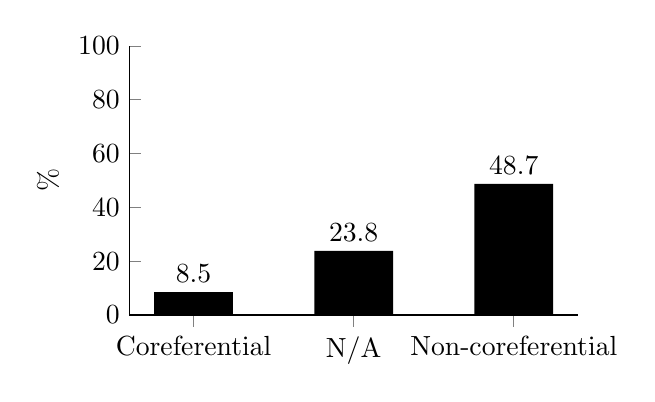
\begin{tikzpicture}
    \begin{axis}[
            ybar,
            ylabel={\%},
            xtick=data,
            axis lines*=left,
            ymin=0,
            ymax=100,
            width=.6\textwidth,
            enlarge x limits={.2},
            height=5cm,
            bar width=1cm,
            nodes near coords,
            nodes near coords style={text=black},
            xticklabels={{Coreferential}, {N/A}, {Non-coreferential}},
            ]
            \addplot[fill=black,draw=none] coordinates {(0,8.5) (1,23.8) (2,48.7)};
    \end{axis}
\end{tikzpicture}
\end{figure}

Interestingly, our results also reveal that the presence of the overt indirect object strong pronominal form is not only conditioned by the cognitive features of the indirect objects occurring in the preceding discourse but also by the cognitive features of preceding subjects. In this respect, we find that when the referent of the previous subject is the same as the referent of the indirect object, \textit{a min\slash a mí} is disfavored in our data. This result suggests that first person singular pronouns are interrelated in the discourse regardless of the syntactic function (indirect object, subject) they fulfill in the clause. 

\subsection{Interactional factors} 
The quantitative analyses summarized in \tabref{tab:brown:2} reveal a significant effect of utterance position on expression\slash omission of \textit{a min\slash a mí}. When the indirect object clause follows a pause (as indicated in the orthographic transcriptions), the expression of the strong pronoun is favored as compared to when the clause is embedded elsewhere in the discourse. This result is independent of the role that the subject reference of the previous clause plays in \textit{a min\slash a mí} expression. In most cases (72\%, $N=440$), when the target clause occurs after a pause, the reference of the indirect object is different from the reference of the subject of the previous clause. However, within switch reference contexts, the percentage of \textit{a min\slash a mí} expression is significantly higher ($p < 0.0000,\allowbreak \chi^2 = 22.48862$) when it occurs in a clause following a pause (28\%, $N=123$) than when it occurs in other interactional positions (15\%, $N=69$). This result suggests that, regardless of reference-tracking factors, the occurrence of expressed \textit{a min\slash a mí} may also be conditioned by an interactional effect.\footnote{An anonymous reviewer suggests that an interpretation of this result is that the speaker is orienting the interpretation of subsequent discourse as specifically regarding his/her perspective (e.g., \citealt{FauconnierTurner2006}).}  As is noted by \citet[737]{TravisTorresCacoullos2012} with regard to overt \textit{yo}, this interactional effect may well have led to the traditional interpretations of contrast and emphasis associated with the expression of strong pronominal forms in object function. 

This finding also suggests a potential role for Intonation Units (IUs) (\citealt{DuBoisPaolino1993}) in constraining indirect object pronominal expression in line with results reported for subject pronominal expression (\citealt{TravisCacoullos2012, TorresCacoullosTravis2014}). Future research on corpora that are IU-transcribed may be able to ascertain if the same pattern holds true for indirect objects.

\subsection{Constructional factors}

\begin{table}[ht]
\begin{tabular}{lrr}
\lsptoprule
{Verb infinitive} & \multicolumn{1}{c}{$N$} & \multicolumn{1}{c}{\% expression}\\\midrule
\textit{pasar} ‘happen’ & 26 & 61.5\\
\textit{importar} ‘matter’ & 24 & 54.2\\
\textit{soar\slash sonar} ‘sound’ & 12 & 33.3\\
\textit{parecer} ‘seem’ & 108 & 25.9\\
\textit{encantar} ‘love’ & 50 & 24.0\\
\textbf{\textit{gustar}} ‘like’ & 289 & 23.5\\
\textit{dar} \textit{pena,} etc. ‘cause pain’ & 46 & 21.7\\
\textit{ocorrer\slash ocurrir} ‘occur’ & 15 & 20.0\\\hdashline
\textit{falar\slash hablar} ‘speak’ & 11 & 18.2\\
\textit{saír\slash salir} ‘leave’ & 11 & 18.2\\
\textit{dar} ‘give’ & 67 & 11.9\\
\textit{custar\slash costar} ‘cost’ & 10 & 10.0\\
\textit{tocar} ‘to be one’s turn’ & 33 & 9.1\\
\textit{quedar} ‘have left’ & 11 & 9.1\\
\textbf{\textit{dicir} \textbf{/} \textbf{decir}} \textbf{‘say’} & 178 & 5.6\\
\textit{contar} ‘tell’ & 25 & 4.0\\
\textit{facer\slash hacer} ‘do, make’ & 25 & 4.0\\
\textit{poñer\slash poner} ‘put’ & 15 & 0.0\\
\textit{quitar} ‘remove’ & 10 & 0.0\\
\lspbottomrule
\end{tabular}
\caption{Rates of overt \textit{a min/a mí} expression in translation equivalents occurring 10+ more times in data\label{tab:brown:4}}
\end{table}

Our quantitative analysis indicates that intransitive constructions (i.e., grammatical patterns) favor expression of the strong indirect object pronoun over (di)transitive constructions. Similarly, \citet{OrozcoHurtado2021} have also shown that syntactic construction significantly constrains subject pronoun expression in Spanish. In order to determine whether all verbs within these two categories behave similarly or not, we examine rates of expression for each translation equivalent with 10 or more tokens in our data. \tabref{tab:brown:4} summarizes our findings. We group together Galician and Spanish forms (for example, \textit{soar} and \textit{sonar} ‘to sound’, are considered jointly). Recall, the average rate of overt \textit{a min\slash a mí} expression is 19\% (see \tabref{tab:brown:1}). We have approximated this in the table with a dotted line. All verbs listed above the dashed line have rates of expression higher than 19\%, and those below have lower than average rates. The two bolded types in the list (\textit{gustar, dicir\slash decir}) are the two verbs with the highest token frequency in each category (intransitive and (di)transitive respectively). The rates of expression for these two particular verbs differ significantly ($\chi^2 = 25.40103, p < 0.000$), with \textit{gustar} exceeding the average (23.5\%) and \textit{dicir\slash decir} falling well below the average (5.6\%). The high token frequency verb \textit{dicir\slash decir} has remarkably low rates of overt strong pronoun expression and may work to suppress the rates of expression in the whole category (along with other speech verbs such as \textit{contar} and \textit{hablar}). 

The verbs with greater than average rates of \textit{a min\slash a mí} expression (among our most frequent types), belong to the same semantic category along with \textit{gustar}. Previous studies \parencites[101]{DelbecqueLamiroy1996}[1879]{GutiérrezOrdoñez1999} include these verb types into the category of “psych-movement” or “psychological verbs”. Again, here, we can see a parallel with the literature on subject (as opposed to object) pronoun expression. Many studies (e.g., \citealt{Enríquez1984, OtheguyZentella2012, Posio2013, Posio2014, Posio2015, Herbeck2021, TravisCacoullos2021}) report higher rates of overt subject pronouns with cognitive-psych verbs than with other verb types. Usage-based analyses of subject pronoun expression (e.g., \citealt{BrownShin2022}) suggest a verb's history of use conditioning context may help account for the overall higher rate of subject pronoun expression for this verb class. Given the variability apparent in \tabref{tab:brown:4} within the categories of transitive and intransitive (cf. \textit{pasar} 61.5\%, \textit{quedar} 9.1\%), the relative contribution of construction as opposed to verb semantics in predicting strong pronoun expression remains to be determined.

\section{Conclusion}

It has been common practice in linguistics to identify grammatical relations on the basis of coding devices such as case, presence/absence of an adposition, agreement and clausal position. In this line, grammatical relations such as subject, direct object and indirect object have become part of the core metalanguage to describe the structure of (accusative) languages such as Galician and Spanish. Subject, direct object and indirect object can be expressed by means of different grammatical markers including agreement, clitics, strong personal pronouns, and lexical NPs. Undoubtedly, this methodology has contributed enormously to our understanding of linguistic structure. However, by assuming that grammatical relations play a central role in language, we tend to take them as the starting point of our analyses, turning in this way our back to any commonalities that may exist across them. For example, the results of this paper suggest that first person singular behaves similarly across different grammatical relations (indirect object and subject) regarding cognitive, mechanical and interactional factors. Our results also suggest that the expression of first person singular is determined by the occurrence of a first person singular in the preceding discourse, regardless of its grammatical relation. These factors may outweigh syntactic functions in accounting for grammatical variation. Future research might consider giving precedence to grammatical categories (such as first person singular) over grammatical relations in their accounts of processes of language variation and change.


\printbibliography[heading=subbibliography,notkeyword=this]
\end{document} 
